\chapter{相关工作}

\section{需求可追踪性的相关技术}

\subsection{需求可追踪性的基本概念}

在软件工程领域,人们认为应该要追踪一个需求使用期限的全过程,编制每个需求同系统元素之间的联系文档,这样的关联关系提供了需求到产品整个过程范围的明确的查阅能力,需求可追踪性(Traceability)概念的提出,正是为了应对上述问题。1970年,需求可追踪性被列入美国国防部合同条款;1992年,经过软件工程领域内的广泛讨论被认为有助于软件开发实践;1994年,需求可追踪性有了如下的明确定义\cite{gotel1994analysis}:

定义:需求可追踪性是指,在软件生命周期中,对某一特定需求形成以及演变的追踪能力,既包括后向追踪,从需求文档确定后一直到软件发布过程中的各种制品之间的追踪(例如设计文档、代码和测试)又包括前向追踪,书写文档形式的需求追踪到需求的来源。

无论是正向追踪或是反响追踪,我们都可以用一个二维矩阵将对应关系固化。以需求与代码间的追踪关系为例,图N为对应的需求追踪矩阵。其中,列表示需求项,行表示代码项,矩阵间的标记表明对应列的需求与对应行的代码存在关联关系,既此代码负责实现该需求描述的行为,在实际的软件生产过程中,需求的粒度可以是用例(Use Case)或声明(Requirement Statement),对于面向对象的程序,代码的粒度通常是类或者函数。

\begin{table}[]
\centering
\caption{需求追踪矩阵(需求到代码)}
\label{my-label}
\begin{tabular}{@{}cccccc@{}}
\toprule
      & $Requirement_{1}$ & $Requirement_{2}$ & $Requirement_{3}$ & ... & $Requirement_{n}$ \\ \midrule
$Code_{1}$ & X            &              &              &     &              \\
$Code_{2}$ &              & X            &              &     &              \\
$Code_{3}$ & X            &              &              &     & X            \\
$Code_{4}$ &              &              & X            &     & X            \\
...   &              &              &              &     &              \\
$Code_{n}$ &              & X            &              &     &              \\ \bottomrule
\end{tabular}
\end{table}

\subsection{研究现状}

Maeder等人\cite{mader2012assessing}分析了需求可追踪性对于软件维护任务的有益程度,他们通过研究案例iTrust与Gantt的实验,分析认为在需求可追踪性的辅助下,维护任务平均能够提高21\%的效率与60\%的准确度。然而,追踪关系的建立和维护需要也需要成本,只有当收益高于成本时,追踪关系的实施才有现实意义。文章\cite{mader2012assessing}同时分析了收益成本间的关系,分析显示随着软件演化,当维护任务达到一定数量时,在需求可追踪性的辅助下能够减少维护任务的总成本。

尽管如此,真实世界的软件系统中通常缺少固化的追踪关系\cite{ramesh1995implementing},这主要是由于(1)追踪关系在软件开发的过程中难以捕获。要求开发者在实现软件功能的同时建立和维护追踪关系代价较高,开发者实施追踪关系的意愿不高;(2)追踪关系在软件开发完成后难以重建。对于一个完成的软件系统,早期参与的开发者可能已经不在项目组中,或是遗忘系统的实现细节,导致重建追踪关系的困难。因此,领域内希望通过增强过程的自动化程度以辅助开发者完成追踪关系的生成。

目前领域内主流生成追踪关系的方法是从Antoniol等人\cite{antoniol2002recovering}的奠基性工作发展而来,该工作利用基于VSM(向量空间模型)的方法检索需求和代码间的追踪关系。方法核心在于利用信息检索技术估计文本间的相似度。继承这一想法的工作\cite{marcus2003recovering,cleland2005utilizing}分别选用LSI(潜在语义索引),JS(概率模型)检索需求和代码间的追踪关系,而比较三者模型发现,没有一种检索模型占有明显优势\cite{abadi2008traceability,eaddy2008cerberus}。

尽管基于信息检索的方法能够完全自动化的生成追踪关系,但是此类方法的精度(准确率,召回率)有限。这是由于基于文本匹配的信息检索存在词汇失配(Vocabulary Mismatch)的问题。代码的文本质量低,同义词问题等情况都会影响检索的精度。因此,出现了一系列的工作对基于信息检索的追踪关系生成方法进行改进。Dasgupta等人\cite{dasgupta2013enhancing}通过引入与代码相关的文档扩展以扩展文本的内容;Ali等人\cite{ali2012empirical}利用Eye-Tracking设备追踪维护人员在建立追踪时的眼球轨迹,以发现对维护人员重要的代码实体,并根据代码实体的重要性(函数>注释>变量>类)为来自代码实体的词项赋权;在 Ali等人\cite{ali2013trustrace}的另一份工作中,通过挖掘软件生产过程以提供额外的信息源(Commit,Bug Report,Mail List)参与决策
;Mahmoud\cite{mahmoud2013supporting}等人通过重构代码的方式改善了代码文本的质量,以减轻词汇失配的程度。Capobianco\cite{capobianco2013improving}等人则认为在检索时名词能够提供最为关键的信息,而形容词和副词等会带来干扰;Diaz等人\cite{diaz2013using}提出利用代码所有权的概念提高追踪关系的检索精度。

上述方法主要是通过引入额外文本信息或对文本赋权的方式以弥补原有需求、代码文本质量的不足。而代码与需求不同,除了文本信息之外,代码还包含结构信息,另一类工作通过深入挖掘代码的结构信息以提高追踪关系的检索精度。McMillan等人\cite{mcmillan2009combining}结合代码的文本和结构信息用于追踪关系的生成,在基于文本信息检索的候选追踪关系之上,利于结构信息进行追踪关系的重排序;Panichella等人\cite{panichella2013and}认为如果候选追踪关系本身的精度较低,则基于代码结构信息的重排序可能起到反效果,因此提出在用户反馈阶段使用代码结构信息。

\subsection{基于信息检索的需求到代码间追踪关系生成技术}

在需求与软件过程的各种制品之间的关联关系中,需求与代码的关联关系引起了开发者的主要关注,这是由于需求描述了与软件系统行为有关的高层概念,而代码负责软件系统行为的实现,两者的关联关系能够帮助开发者理解程序,分析需求变更的影响性,完成包括维护任务、二次开发,代码复用在内的一系列软件活动。

\begin{figure}[thb]
    \centering
    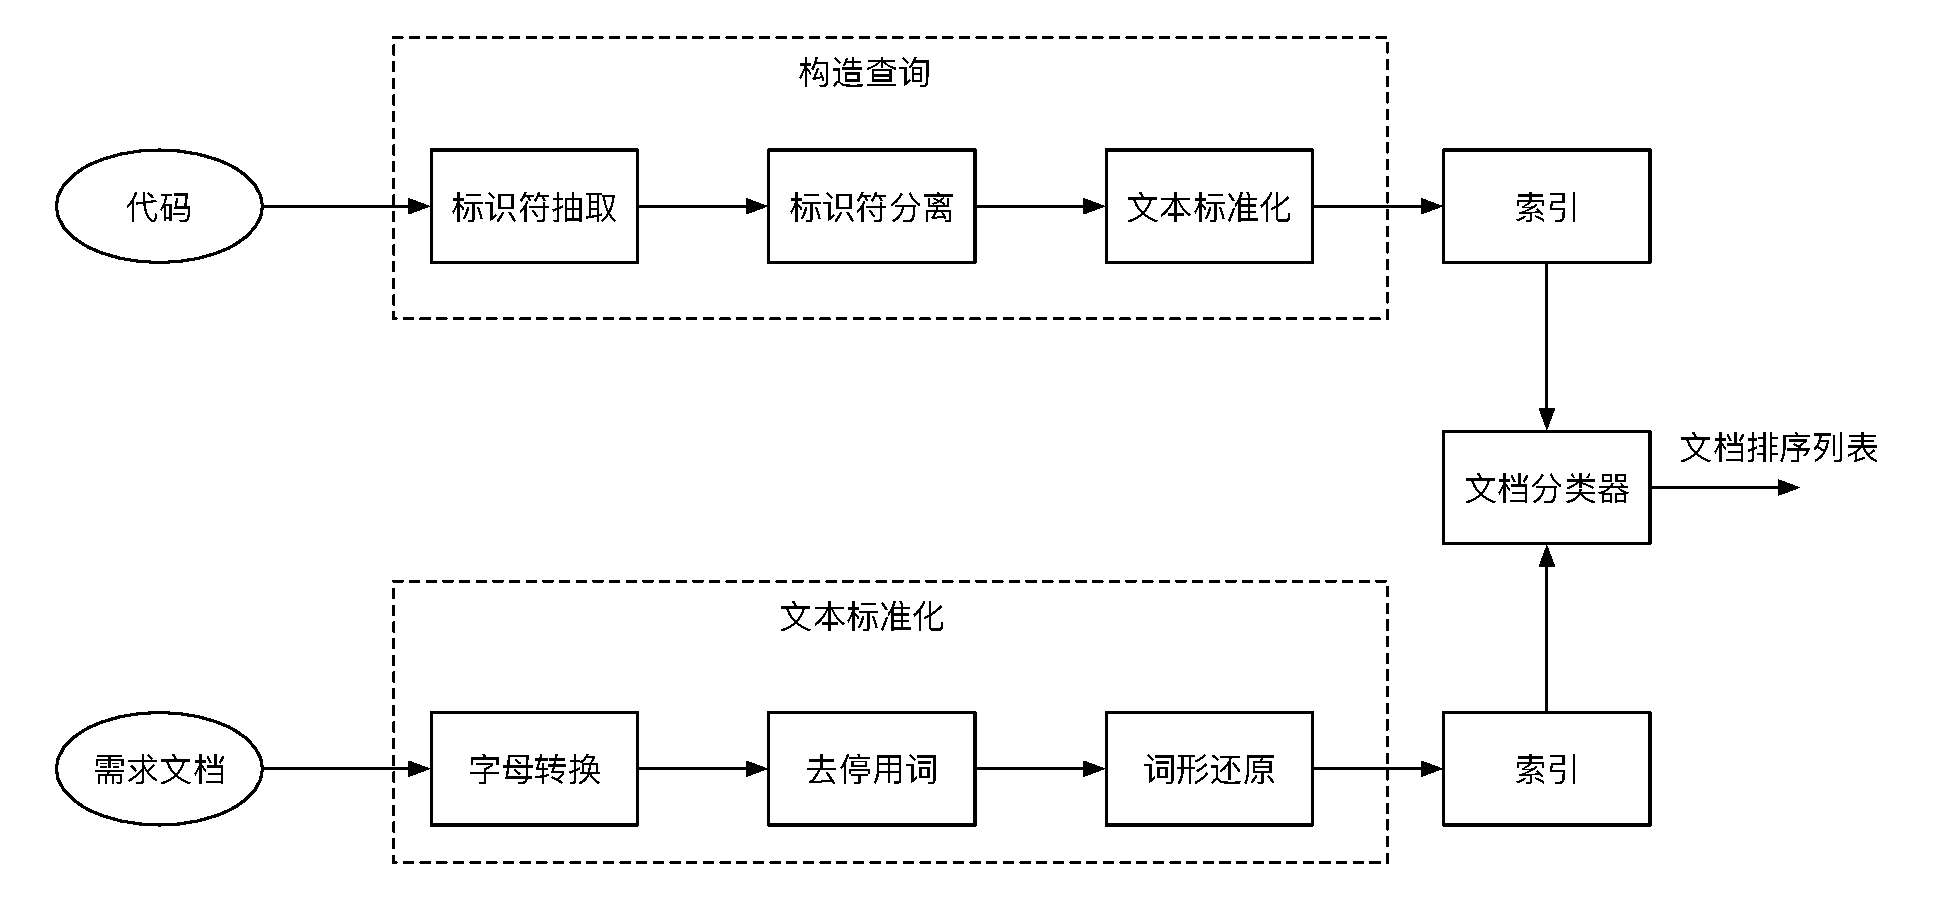
\includegraphics[width=1.0\textwidth]{./figures/related_work/ir_traceability_process.pdf}
    \caption{追踪关系生成方法}
    \label{F:BuildLogScrn}
\end{figure}

% \subsection{追踪关系生成方法}

Antoniol等人\cite{antoniol2002recovering}提出了基于信息检索的需求到代码间追踪关系生成方法。方法的核心想法是,假设代码中标识符的命名有意义,或与需求文档共用同一个术语表,因此能够通过文本匹配的方式建立需求和代码的关联关系。方法的基本过程如图N所示。在进行需求和代码的检索前,方法首先通过两条路径(需求文档到文档,代码到查询)构造文档与查询。

在构造文档这一路径,基于文档中抽取的词能够建立文档的索引,词的构造与索引的建立需要通过以下三个步骤的文本标准化处理:
\begin{enumerate}
  \item 将文档中的字母统一转换为小写。

  \item 根据停用词表删去文档中的停用词,通常停用词包括(标点、数字、介词等)。

  \item 词形还原,包括将名词的复数形式转换为单数形式,将包含时态的动词还原为动词原形。
\end{enumerate}
在构造查询这一路径,方法将每个代码组件(通常是类或函数)作为一个查询,查询的构造包括以下三个步骤:
\begin{enumerate}
  \item 解析代码文本,提取代码组件的标识符。

  \item 根据标识符的命名规则(驼峰命名法,下划线分割命名法),将标识符分隔为若干独立词项。例如,标识符AmountDue,amount\_due将被分隔为词amount,due。

  \item 利用对文档进行标准化处理的三个步骤处理文本。
\end{enumerate}
最终,通过文本分类器计算查询和文档间的相似度,并返回需求到代码的候选追踪关系列表,列表根据需求文档和代码的相似度值倒序排列。显然,排序的结果与方法采取的信息检索模型有关,我们将会对三种信息检索模型(VSM,LSI与JS)进行介绍,VSM模型将查询和文档看作向量,文档根据计算的向量间距离排序;LSI在VSM的基础上,通过奇异值分解以识别词句间隐性的关联关系的模式;JS属于概率模型,估计文档与查询相关的概率,对文档根据关联概率进行排序。后续小节中将会对这三个检索模型进行详细阐述。
% \subsection{信息检索模型}

\subsubsection{VSM}
VSM(Vector Space Model)是现代信息检索系统中比较常用的检索模型,它的思想是将文档与查询都看作是高维空间中的一个向量,每个维度都是一个独立的词项。

如果某个词项出现在了文档中,那它在向量中的权重就非零。常见的权重计算方法为TF-IDF,其中,TF(term frequency)是指给定的某一个词项在文本中的出现频率,IDF(inverse document frequency)用于度量词项的普遍重要性。根据直觉,对于查询中的某一个词项,如果在文档A中的出现次数多于文档B,那么文档A比B对于查询更相关。但是这里有一个缺陷在于,内容长的文档比内容短的文档有优势,长的文档总的来讲包含的词项要多些。因此我们根据文档的长度,对词项次数进行归一化,将词项次数除以文档的总词项数,这个商称为“词项的频率”,可以作为词项的局部权重。除了局部权重以外,如果一个词项只在很少的文档中出现,那么通过它就容易定位目标,应该赋予该词项较高的权重。反之,如果一个词项在大量文档中出现,则表明该词项缺少独特性,它的权重就应该较小。我们用“逆文本频率指数”(IDF)来衡量词项的全局权重。TF-IDF的计算公式如下:
\begin{align}
    tf_{i,j}=\dfrac {n_{i,j}} {\sum _{k}n_{k,j}}
  \end{align}
  \begin{align}
    idf_{i}=\log \dfrac {\left| D\right| } {\left| j:t_{i}\in d_{j}\right| }
  \end{align}
   \begin{align}
    tfidf_{i,j}=tf_{i,j} \times idf_{i}
  \end{align}
其中,$tf$指给定的某一个词项在文档中的出现频率。$n_{i,j}$为词项$t_{i}$在文档$d_{j}$中的出现次数,分母表示在文档$d_{j}$中所有词项的出现次数之和;$\left| D\right|$表示文档库中的文档总数,表示包含词项$t_{i}$的文档数目。

相似度计算是基于这样一个假设,词是文本的载体,文本的信息和词的语义是联系在一起的,也就是说同一类文本用词是相似的,不同类的文本用词各不相同。由于向量空间模型将文档与查询都看作是高维空间中的一个向量,查询与文档的相似性可基于它们在向量空间中的夹角来衡量。给定查询向量$q$, 文档向量$d$, 向量长度均为$n$, 那么其余弦相似度定义为:
\begin{align}
    sim(d_{j},q)=\dfrac {\sum _{i=1}^{n}w_{i,j} \times w_{i,q}} {\sqrt {\sum _{i=1}^{n}w_{i,j}^{2}} \ \times \sqrt {\sum _{i=1}^{n}w_{i,q}^{2}}}
  \end{align}
其中,w表示对应文档中由TF-IDF计算而来的词项权重。

\subsubsection{LSI}
LSI(Latent semantic indexing,潜在语义索引)\cite{deerwester1990indexing,dumais1991improving}在VSM的基础上通过分析词句的使用模式,以发现词句间潜在的联系。
LSI在自然语言文本中的应用表明\cite{berry1992large,landauer1997solution},LSI不仅可以捕获独立词语的含义,而且可以捕获短语(词组,句子)的含义。LSI的核心想法是,在同样的语境中出现的词语存在某些相互约束,限定了这些词之间一半具有相似的含义。在经典的文本分析应用中,LSI使用给定的语料创建词项-文档矩阵(Term-by-Document matrix),并采用奇异值分解\cite{salton1986introduction}的方式构造词项-文档矩阵的子空间,称之为LSI子空间。新的查询、文档向量通过将VSM空间的相关向量投影至LSI子空间生成。

奇异值分解背后的形式化较为复杂,详细内容可参考文献\cite{salton1986introduction}。直观来说,奇异值分解能够将一个矩阵分解为三个矩阵的乘积。给定原矩阵$X$,子矩阵$U$是对原矩阵行实体分类的结果,子矩阵$V$是对原矩阵列实体分类的结果,中间的对角矩阵则表示原矩阵行实体与列实体之间的相关性,原矩阵$X$可以被此三个矩阵重建($X$ $=$ $U$$\Sigma$$V^T$)。$U$与$V$的列分别为左奇异向量与右奇异向量,对应的$\Sigma$中单调递减的对角元素称为原矩阵$X$的奇异值。当在重建矩阵过程中只使用部分奇异值因子数时,重建的矩阵是一个最小二乘法拟合。取$U$,$V$的前k列与前k个(最大的)$X$的奇异值时,利用$X_{k}$ $=$ $U_{k}$$\Sigma_{k}$$V_{k}^T$,可以构造$X$的秩-k近似矩阵。$U$与$V$的列是正交的,故$U^TU$ $=$ $V^TV$ $=$ $I_{r}$,其中$r$是原矩阵$X$的秩。$X_{k}$由k个最大的奇异三元组(一个奇异值及与之对应的左右奇异向量为一个奇异三元组)构造而成,称之为原矩阵$X$的k维最佳近似矩阵。

对于LSI而言,构造以关联矩阵$X$形式表示的词项-文档矩阵的k维最佳近似矩阵$X_{k}$。通过矩阵降维的方式,许多导致检索精度不理想的“噪音”能够被消除。为了取得较好的检索效果,选取较高的k值是有必要的。但需要注意的是,k值如果过高,可能导致原矩阵$X$被重建,则词语多样性带来的干扰会造成检索精度的下降。一些研究表明,LSI子空间的维度的选择对LSI的效果有较大的影响\cite{deerwester1990indexing,dumais1991improving,dumais1994latent}。在实际中,维度的选择通常由实验确定,或是参考已有工作以确定。新的查询、文档向量通过将VSM空间的相关向量投影至LSI子空间生成,查询与文档间的相似度可以由对应向量间的余弦距离计算确定。

\subsubsection{JS}
JS模型(Jensen-Shannon similarity model)是较新的一种信息检索技术,属于概率模型。在概率模型中,假设每一个查询与文档都包含一个潜在的概率分布,则文档的排序可以由概率分布间的距离确定。JS相似性模型将查询与文档看作词项的概率分布,概率分布间的差异度量可以由JS散度计算\cite{cover2012elements}而得,定义如下:

\begin{align}
 JS(q,d) \triangleq H(\dfrac {\hat {p}_{q}+\hat {p}_{d}} {2}) - \dfrac {H(\hat {p}_{q})+H(\hat {p}_{d})} {2}
  \end{align}
  \begin{align}
 H(p) \triangleq \sum _{w\in W}h(p(w)),\ h(x) \triangleq -x\log x
  \end{align}

其中,$H(p)$表示概率分布$p$的熵,$\hat {p}_{q}$与$\hat {p}_{q}$分别表示查询与文档的概率分布。根据定义可知,$h(0) \equiv 0$,故定义查询与文档间的相似度得分为$1 - JS(q,d)$。

\subsection{结合代码文本与结构信息的追踪关系生成方法改进}

由于词汇的多义性,代码的标识符脱离了所处的上下文信息容易具有误导性,代码注释过期\cite{anquetil1998assessing}等情况的存在,相关的代码与需求的文本相似度可能较低。在本小节中,将介绍利用代码结构信息(函数调用,继承关系)改进追踪关系生成方法的相关工作\cite{mcmillan2009combining,panichella2013and,scanniello2015link}。在基于文本匹配的候选追踪关系生成后,此类方法利用代码结构信息对候选追踪关系进行重排序。

\subsubsection{O-CSTI}

McMillan等人\cite{mcmillan2009combining}首先提出利用代码结构信息对候选追踪关系进行重排序方法。给定需求实体(例如,用例)的集合S,代码类的集合$C = \{C_{1}, \cdots, C_{n}\}$,$E = \{(c_{i}, c_{j})\}$,其中$c_{i}$与$c_{j}$间存在依赖关系表示。对于某一给定的需求$s$,从列表中的追踪关系$(s, c_{1})$开始,如果任意$c_{j}$与$c_{1}$存在依赖关系,则给予追踪关系$(s, c_{j})$的相似度值奖励$\delta$(常数或变量)。算法对列表中所有的追踪关系进行同样的处理,并最终根据新的相似度值对列表进行重排序,过程参见算法N。

\begin{algorithm}[htbp]
\caption{Optimistic Combination of Structural and Textual Information — O-CSTI}
\label{alg:O_CSTI}
    $i$ $\leftarrow$ 1\\
    \While {not end of $List$}
    {
      Get the link ($s$, $c_{j}$) in position i of List\\
      \ForAll {$c_{t} \in C$} {
        \If {$(c_{j}, c_{t}) \in E$} {
          Sim($s$, $c_{t}$) $\leftarrow$ Sim($s$, $c_{t}$) + $\delta$ $\times$ Sim($s$, $c_{t}$)
        }
      }
      $i$ $\leftarrow$ $i$ + 1\\
    }
    Reorder List\\
    The user classifies the links in $List$
\end{algorithm}

\subsubsection{UD-CSTI}

在O-CSTI的基础上,Panichella等人\cite{panichella2013and}认为利用代码依赖关系进行的重排序受制于信息检索方法的精度,如果初始的候选追踪关系排序本身质量较低,那么重排序可能会引入更多的错误。因此,作者认为应该在用户反馈阶段执行基于代码依赖关系的重排序,改进后的算法参见算法N。同时,作者在文章中提出了一种自适应的奖励计算方式:$\delta = median\{v_{i}, \cdots, v_{n}\}$。其中$vi = (max_{i} - min_{i}) / 2$,$v_{i}$表示第i个实体相似度值的可变性,$max_{i}$与$min_{i}$表示实体i检索结果中相似度的最高值与最低值。

\begin{algorithm}[htbp]
\caption{User-Driven Combination of Structural and Textual Information — UD-CSTI}
\label{alg:UD_CSTI}
    \While {not (stopping criterion)} 
    {
      Get the link ($s$, $c_{j}$) on top of List\\
      The user classifies ($s$, $c_{j}$)\\
       \If {$s$, $c_{j}$ is correct}
       {
          \ForAll {$c_{t} \in C$} {
            \If {$(c_{j}, c_{t}) \in E$} {
              Sim($s$, $c_{t}$) $\leftarrow$ Sim($s$, $c_{t}$) + $\delta$ $\times$ Sim($s$, $c_{t}$)
            }
          }
       }
      Reorder List\\
      Hide links already classified
    }
\end{algorithm}

\subsubsection{PageRank}
根据代码依赖关系,Scanniello等人\cite{scanniello2015link}利用PageRank算法计算代码的结构重要性,并将需求与代码的文本相似性与该代码的结构重要性的乘积作为排序的依据。

\section{过时需求自动检测的相关技术}

在软件维护和演化的过程中,一份最新的需求规约能够提供有价值的信息以辅 助维护人员完成相应的软件活动。例如,需求规约包含系统实现背后的原理,因此可以帮助维护人员理解程序,或是防止重要的决策被意外忽视。另外,需求规约通常由自然语言文本描述,可以作为用于和软件工程领域外的利益相关者讨论功能更改的基础。因此,当需求规约内的信息变得过时且不可靠时,将减弱系统的可维护性。最终,系统将会进入“维修阶段”(servicing stage)\cite{bennett2000software},此时只可能对系统进行较少且次要的更改。

事实上,在系统演化时,维护人员通常不会及时更新需求规约\cite{bennett2000software,lethbridge2003software},这主要是由于需求的更新仍然需要人工参与,代价高昂,并伴随相应的时间成本。在实践中,维护人员需要查阅可能成百上千页的需求规约,才能够定位其中需要更新的部分。因此,根据Lethbridge等人\cite{lethbridge2003software}的观察,维护人员在面临维护或演化任务时,通常直接更新代码,而不更新相应的需求。很快,需求规约将会变得过时且失效。

\subsection{过时需求的基本概念}

在本小节,我们将阐述过时需求,受影响需求,被检测需求这三者的概念与它们之间的联系\cite{ben2015supporting}。当一个属于需求规约的需求不再反映利益相关者当前的需要时,则该需求被认为是过时的。当维护人员实施一次代码变更后,导致需求规约中的一个或一组需求与新版本的代码不一致时,则这一个或一组需求是受变更影响的需求。当代码变更是用于满足利益相关者新的需要(或是已有需要的改变)时,则受影响需求同时也是过时的。然而,这两类的需求并不是完全重叠的。例如,由于利益相关者的需要发生了改变,则某个需求可以是过时需求,但代码并没有(或是此刻没有)发生更改,因此该需求不是受影响需求。相反的,如果在实施代码变更时没有进行事先的影响性分析,则代码变更很有可能影响某些需求,尽管它们并不过时。然而,在一个管理良好的软件演化过程中,代码通常与利益相关者的需要保持一致,因此过时需求与受影响需求存在很大程度上的重叠(如图N所示)。过时需求自动检测方法通过在代码变更时自动检测受影响需求,从而帮助维护人员识别需求规约中的过时需求。维护人员需要查看这些被检测需求以更新需求规约。在理想情况下,所有受影响需求都应该被检测到。然而,目前过时需求自动检测包含自动分类、检索等步骤,因此方法会存在误报(检测到不受影响的需求)和漏报(受影响的需求未被检测到)的情况。

\begin{figure}[thb]
    \centering
    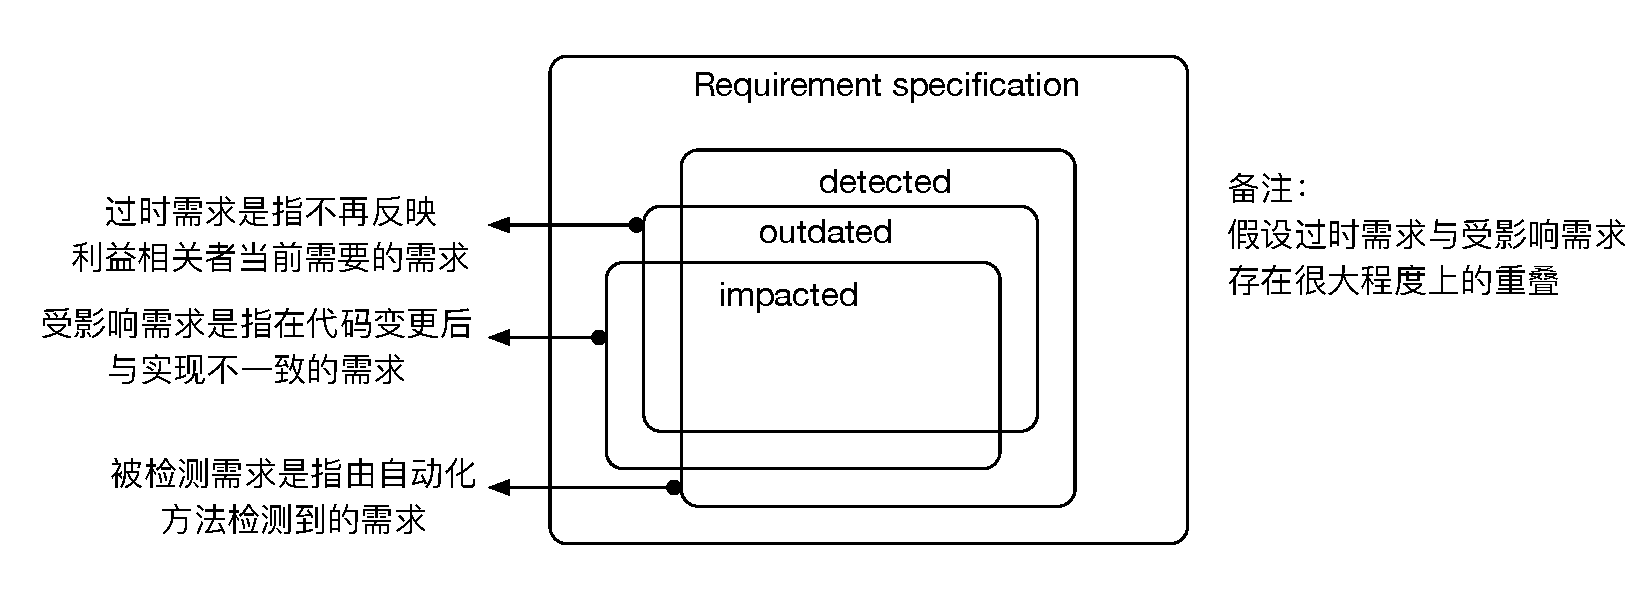
\includegraphics[width=1.0\textwidth]{./figures/related_work/outdated_requirements.pdf}
    \caption{过时需求,受影响需求与被检测需求}
    \label{F:outdated_requirements}
\end{figure}

\subsection{基于代码变更的过时需求自动检测方法}

在软件系统开发的过程中,将创建各种不同的软件实体,其中,代码在软件系统的行为需要发生改变时,会被进行相应的变更。 这是由于如果代码没有发生变更,那么软件系统的行为不会有实际的变化。在实施一次代码变更时,需要执行代码层的影响性分析以识别其中需要被修改的部分。因此,过时需求自动检测方法\cite{ben2015supporting}利用执行代码层影响性分析的过程自动化检测需求中受影响的部分。

在维护人员提交代码变更后,过时需求自动检测方法能够检索潜在受影响需求的排序列表,以供维护人员核查,维护过程参考活动图N\cite{ben2015supporting}。在实施代码变更(A1)并提交至版本控制系统后(A2),代码变更将被自动化分析以判断这些代码变更是否影响需求(A3)。如果检测到影响需求的变更,则利用这些代码变更追踪需求规约(A4),然后将相关的需求以排序列表的形式向维护人员展示(A5),维护人员查看整个候选列表以确定其中的过时需求,并实施更新(A6)。

\begin{figure}[thb]
    \centering
    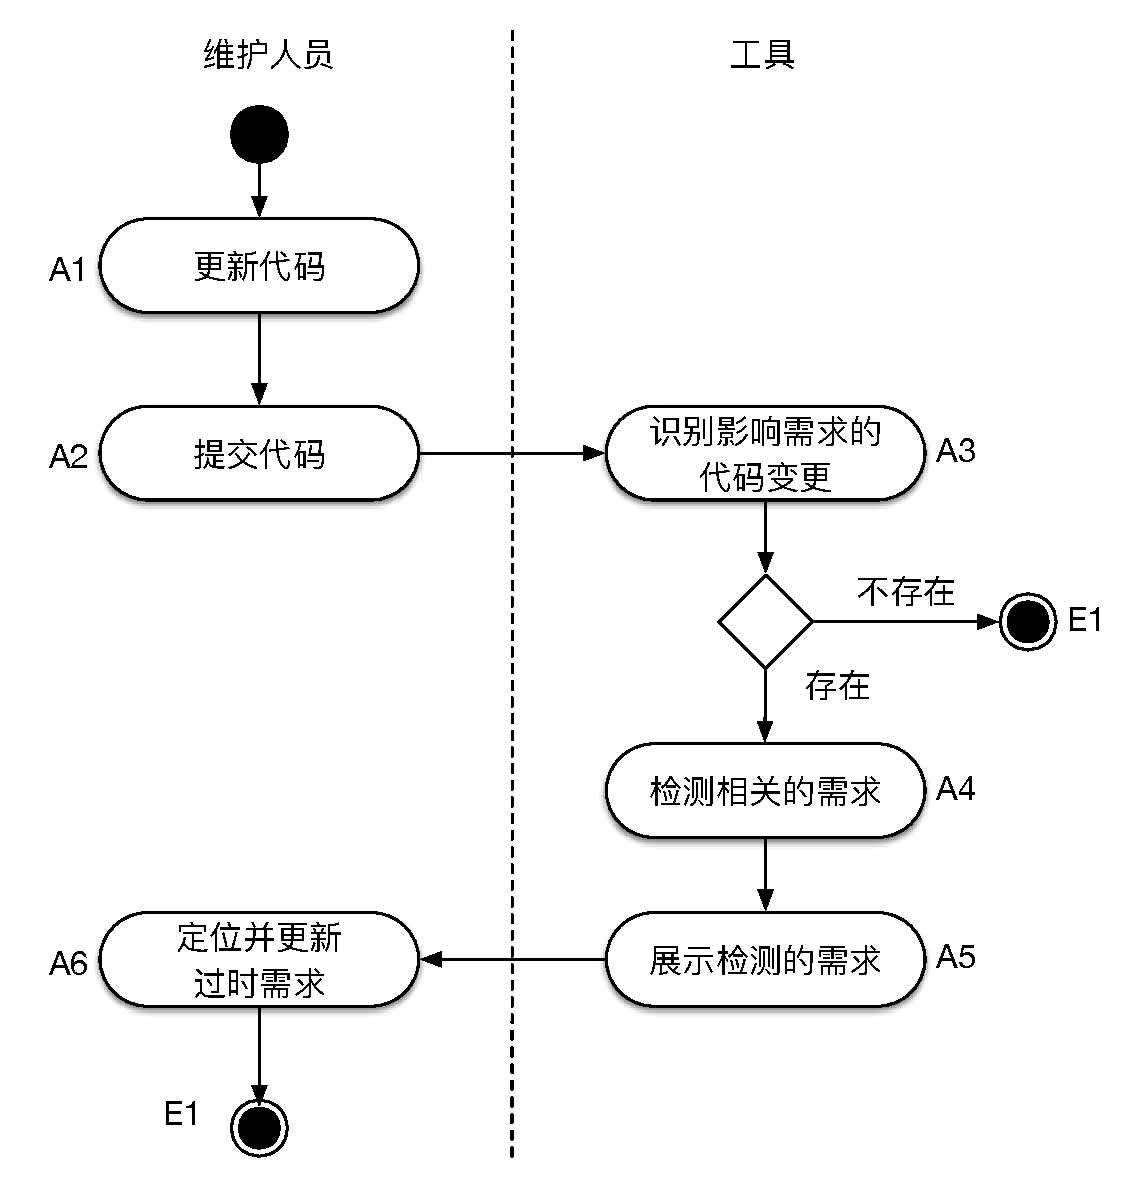
\includegraphics[width=0.7\textwidth,height=0.4\textheight]{./figures/related_work/ActivityDiagram.pdf}
    \caption{活动过程:利用过时需求自动检测方法的维护过程}
    \label{F:ActivityDiagram}
\end{figure}

从实现角度出发,基于代码变更的过时需求自动检测包括三个步骤:(1)识别影响需求的代码变更;(2)检测受变更影响的需求;(3)向用户展示检测的需求。

\subsubsection{识别影响需求的代码变更}
影响需求的代码变更是指,该代码变更能够影响系统的预期行为,或是能够影响系统组件处理外界刺激,数据或功能的反馈\cite{glinz2007non}。Charrada等人通过人工比较ZXing项目1.6与1.7版本的区别,提出了以下六点观察,并根据观察提炼了相应的启发式规则:
\begin{enumerate}
  \item 函数体内的代码变更,多数与重构、缺陷修复有关。因此,忽略函数体内的变更;
  \item 新增或删除代码元素(包、类、函数、域)通常与系统功能的新增或扩展有关。因此,代码元素的新增或删除可能影响系统的外部行为;
  \item 删除某一代码元素,并增加一个与其命名相似的元素,通常是重构(Rename)操作。因此,忽略与Rename有关的代码变更;
  \item 函数签名的变更通常是重构操作。因此,忽略函数签名的变更;
  \item 私有代码元素的变更会影响系统的外部行为。
  \item 多个函数拥有同一个命名(函数重载),通常他们与同一需求有关。因此,只选取其中一个函数进行分析。
\end{enumerate}

根据上述观察得出的启发式规则,方法通过比较代码版本差异,识别其中的变更代码元素(包、类、函数、域),并过滤其中与Rename操作有关的变更。Rename操作可以基于新增和删除的代码元素标识符间文本相似性来判断,相似性可通过编辑距离\cite{levenshtein1966binary}等方式求得。

\subsubsection{检测受变更影响的需求}
根据步骤一中影响需求的代码变更,方法将抽取与代码变更有关的关键词,并利用关键词以追踪需求,生成受变更影响的需求排序。

\section{本章小结}

% \bibliography{reference}